\label{par:etude_diff_rock4}
Pour observer ce qui se produit lorsque l'erreur n'est pas saturée en espace mais que l'erreur temporelle intervient également, 
le logiciel Ponio \footnote{\href{https://github.com/hpc-maths/ponio}{https://github.com/hpc-maths/ponio}} a été couplé à Samurai.
Il permet d'utiliser facilement des méthodes d'intégration en temps complexe. 
Grâce Ponio, l’expérience précédent à été réitérée en remplaçant la méthode ERK2 par la méthode stabilisée ROCK4 \cite{AbdulleMedovikov2001}. 
Cette méthode reste explicite (ce qui permet grâce à Samurai d'étudier facilement les différentes façons d'évaluer les flux) 
tout en assouplissant significativement la contrainte de stabilité.
\subsubsection{Résultats numériques}
    Les résultats sont présentés en fig. \ref{fig:convergence_diffusion_rok4}. Chaque graphique correspond à un paramétrage différent de l'MRA. 
    Les solutions sont comparées à une solution convergée en temps afin d'isoler les erreurs temporelles et celles liées à la MRA de l'erreur spatiale.
    La grille la plus fine du maillage de niveau 12, ce qui correspond à $2^{12}$ cellules et le maillage peut être représenté sur 6 niveaux, donc du niveau $12$ au niveau $12-6=6$.
    Le graphique de droite correspond à un seuil de compression modéré ($\varepsilon = 10^{-5}$) et celui de gauche à un seuil de compression plus restrictif ($\varepsilon = 10^{-6}$).
    Sur chaque graphique l'erreur $L^2$ est tracée en fonction du pas de temps pour chaque méthode de calcul du flux numérique:
{\contour{black}{\textcolor{antiquewhite}{{sans MRA (grille fine)}}}} ;
{\contour{black}{\textcolor{crimson}{{MRA niveau courant}}}} ;
{\contour{black}{\textcolor{peru}{{reconstruction d'un niveau}}}} ;
{\contour{black}{\textcolor{navy}{{reconstruction au niveau le plus fin}}}}.
    Les principales observations sont:
    \begin{enumerate}
        \item Pour un petit pas de temps: plus les flux sont reconstruit finement plus l'erreur augmente, ce qui est étonnant mais cohérent avec l'expérience numérique précédente.
        \item Pour un grand pas de temps: la méthode d'évaluation du flux importe peu. Les erreurs en temps dominent les erreurs liés à la MRA.
        \item Il existe une gamme de pas de temps intermédiaires où les méthodes reconstruisant les flux sur-performent la MRA classique \textbf{et} (étonnant !) la méthode sur grille fine.
    \end{enumerate}
\begin{figure}[h!]
    \centering
    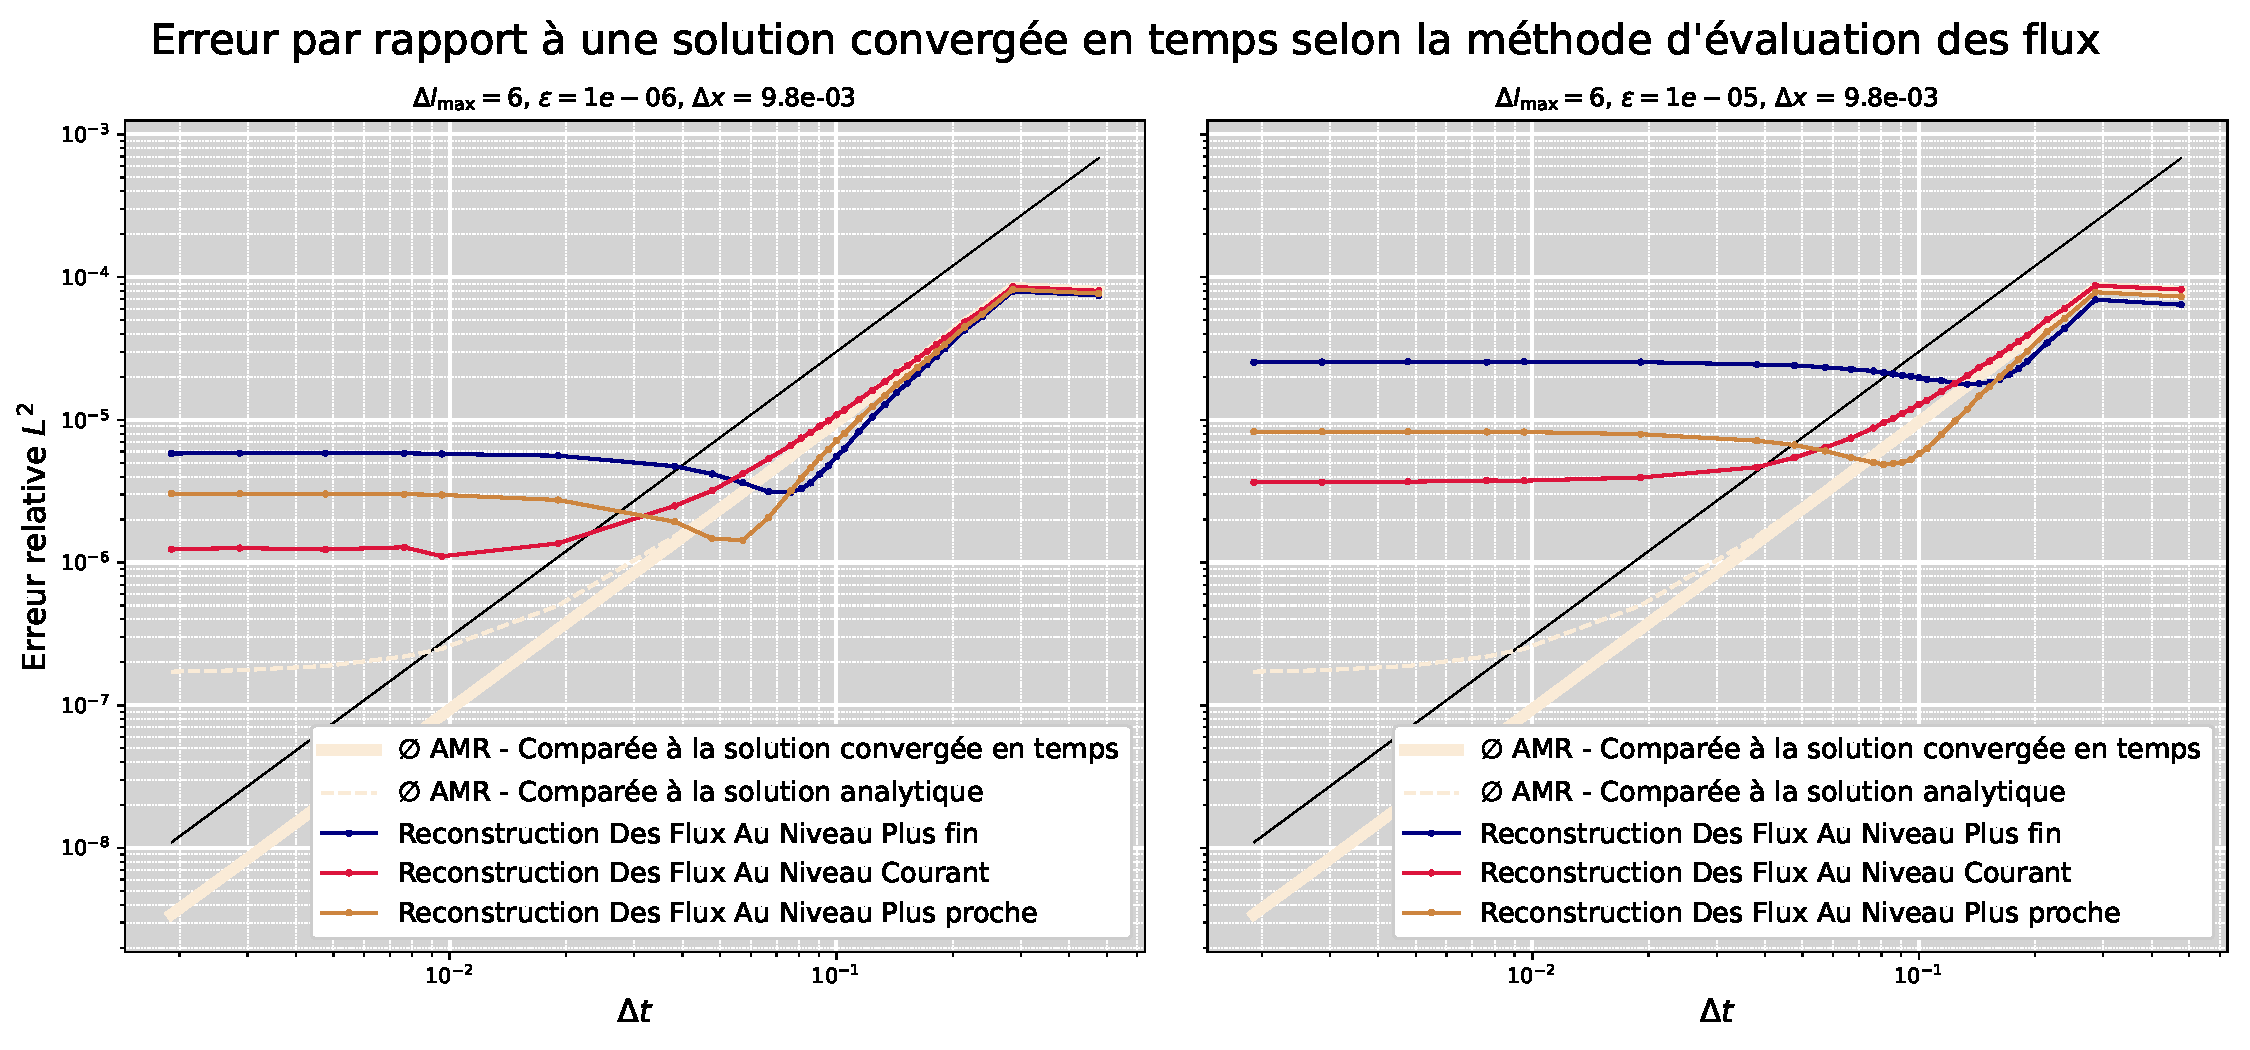
\includegraphics[width=\textwidth]{media/4_travail/3/flux_reconstruction_method_diffusion.pdf}
    \caption{THE CAPTION}
    \label{fig:convergence_diffusion_rok4}
\end{figure}
    Afin d'éclairer ces résultats surprenants, la figure \ref{fig:error_profiles_landscape} présente le profil des erreurs pour les différents régimes de pas de temps: petit, intermédiaire, grand.\par
    \textbf{Pour la méthode sur grille fine et la méthode MRA classique :} le profil présente une \textit{cloche centrale} qui "s'écrase" au fur et à mesure que le pas de temps se réduit, de fait l'erreur chute avec le pas de temps.\\
    \textbf{En revanche pour les méthodes impliquant une reconstruction:} le profil présente également une \textit{cloche centrale} mais au lieu de s'écraser,
    elle change progressivement de convexité et de signe.
    Elle est d'abord positive convexe pour les grands pas de temps puis concave négative pour les petits pas de temps.
    Pour un régime intermédiaire, la cloche est aplatie en zéro ce qui provoque pour ces pas de temps, la chute brutale de l'erreur.\par
    Ce comportement très intéressant - le changement de signe de la cloche - résulte du couplage entre les erreurs en temps du schéma et les erreurs de la reconstruction de la MRA. 
    Dans la suite, nous allons relier cette observations au équations équivalentes précédemment établies.
\clearpage
\begin{figure}[p]
\centering
\rotatebox{90}{%
\begin{minipage}{\textheight}
\centering
\begin{subfigure}{0.32\textwidth}
    \centering
    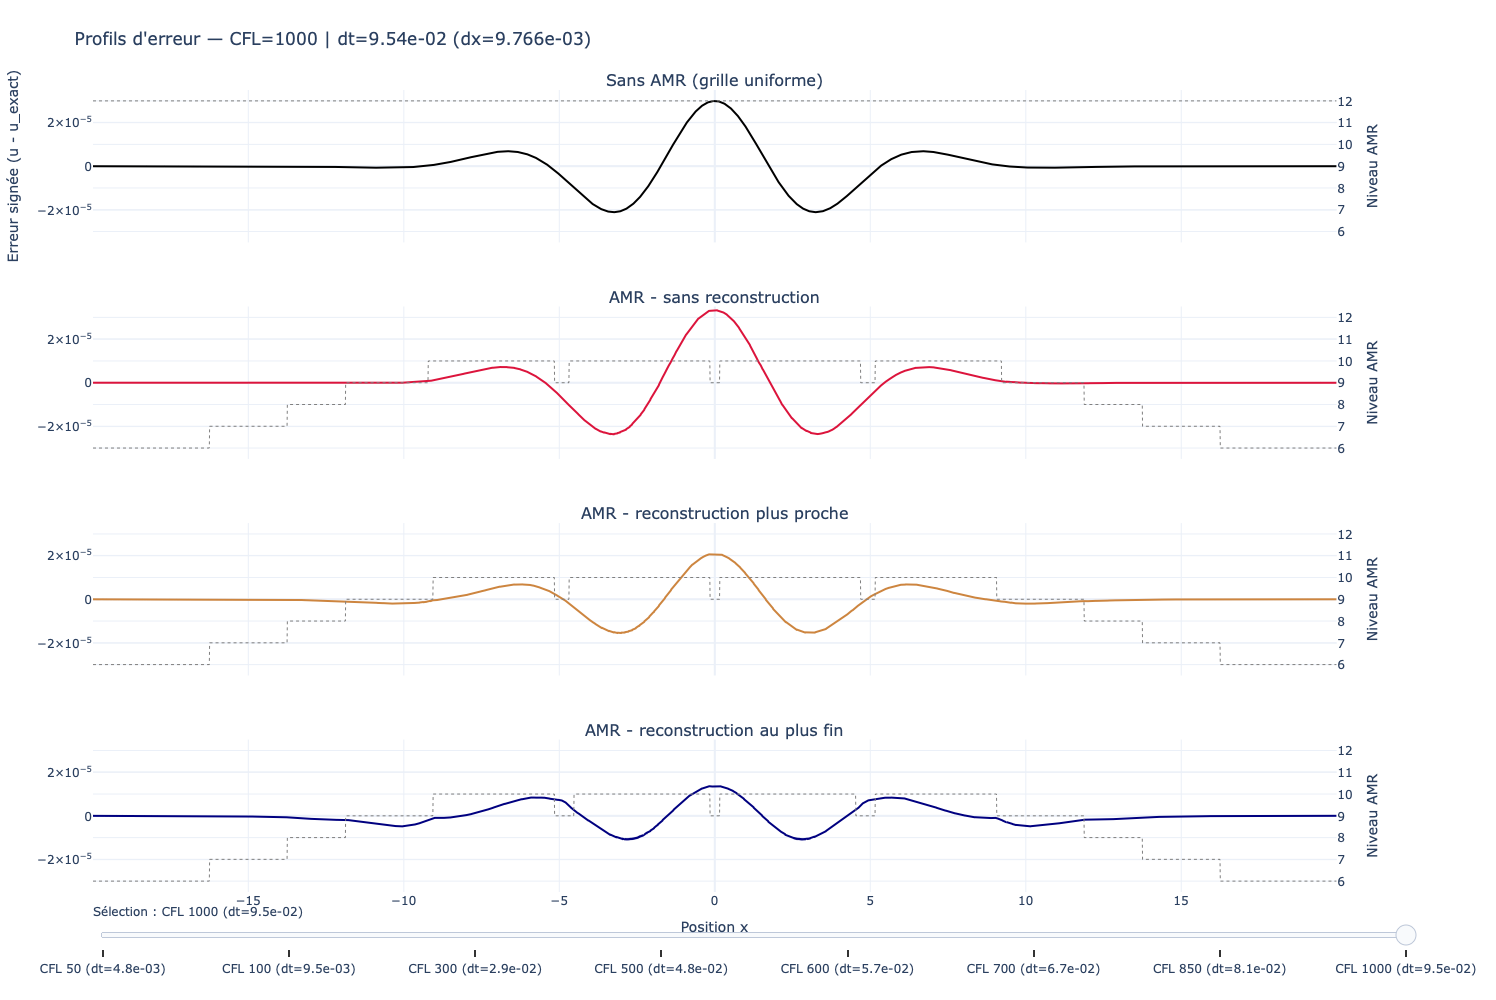
\includegraphics[width=\linewidth]{media/4_travail/3/01_error_profile_big_cfl.png}
    \subcaption{Constante CFL Élevée}
\end{subfigure}\hfill
\begin{subfigure}{0.32\textwidth}
    \centering
    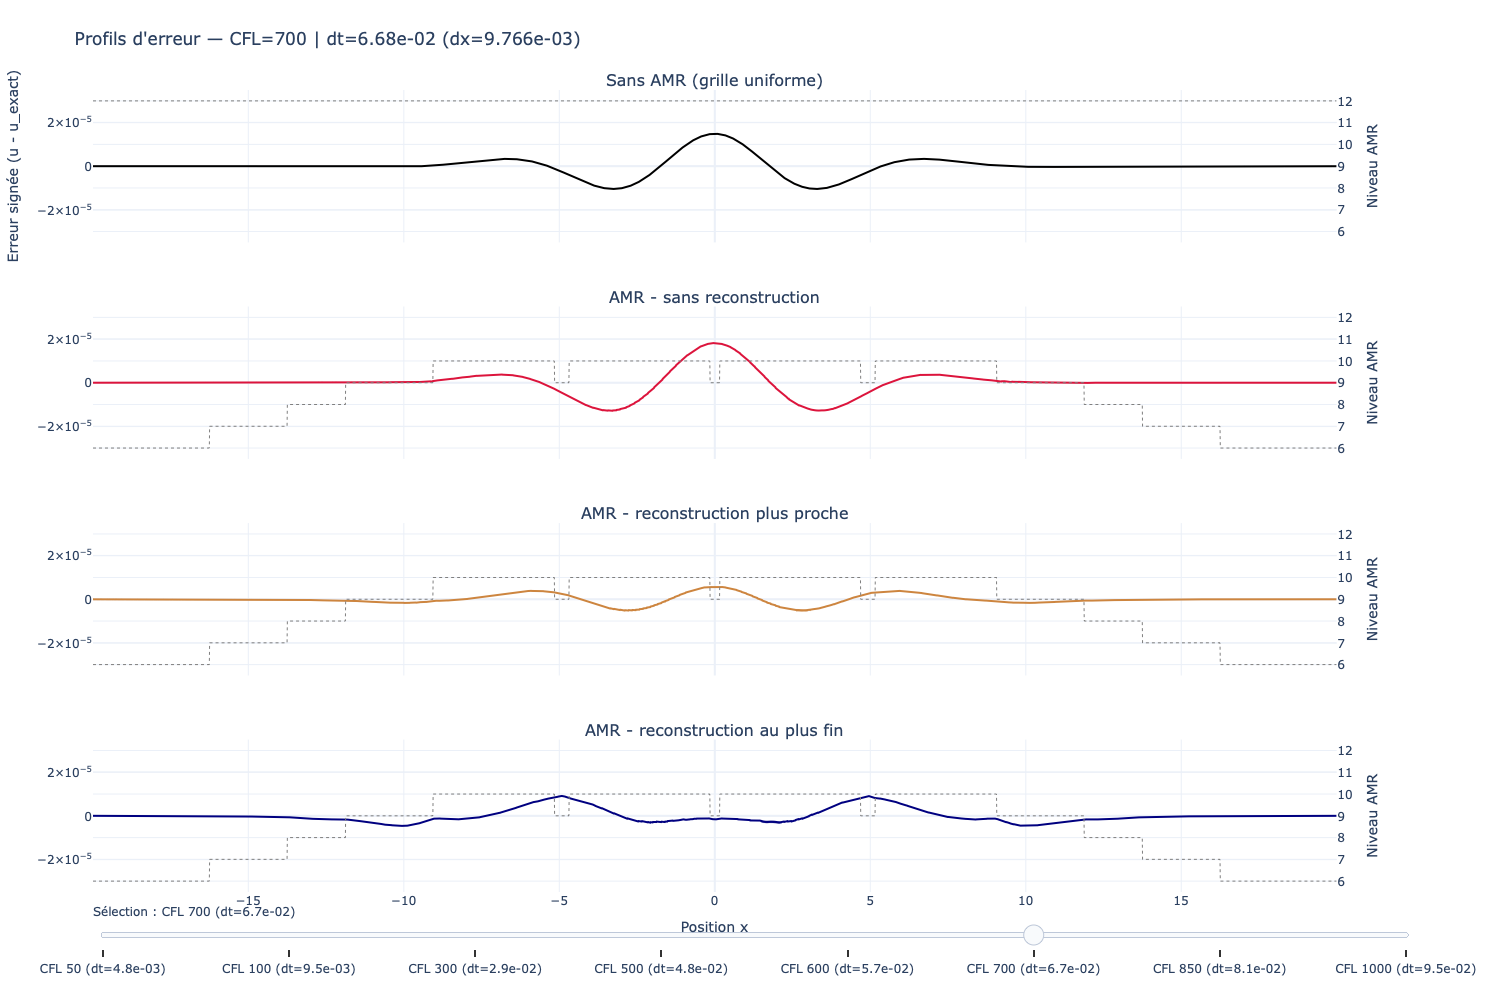
\includegraphics[width=\linewidth]{media/4_travail/3/02_error_profile_medium_cfl.png}
    \subcaption{Constante CFL Moyenne}
\end{subfigure}\hfill
\begin{subfigure}{0.32\textwidth}
    \centering
    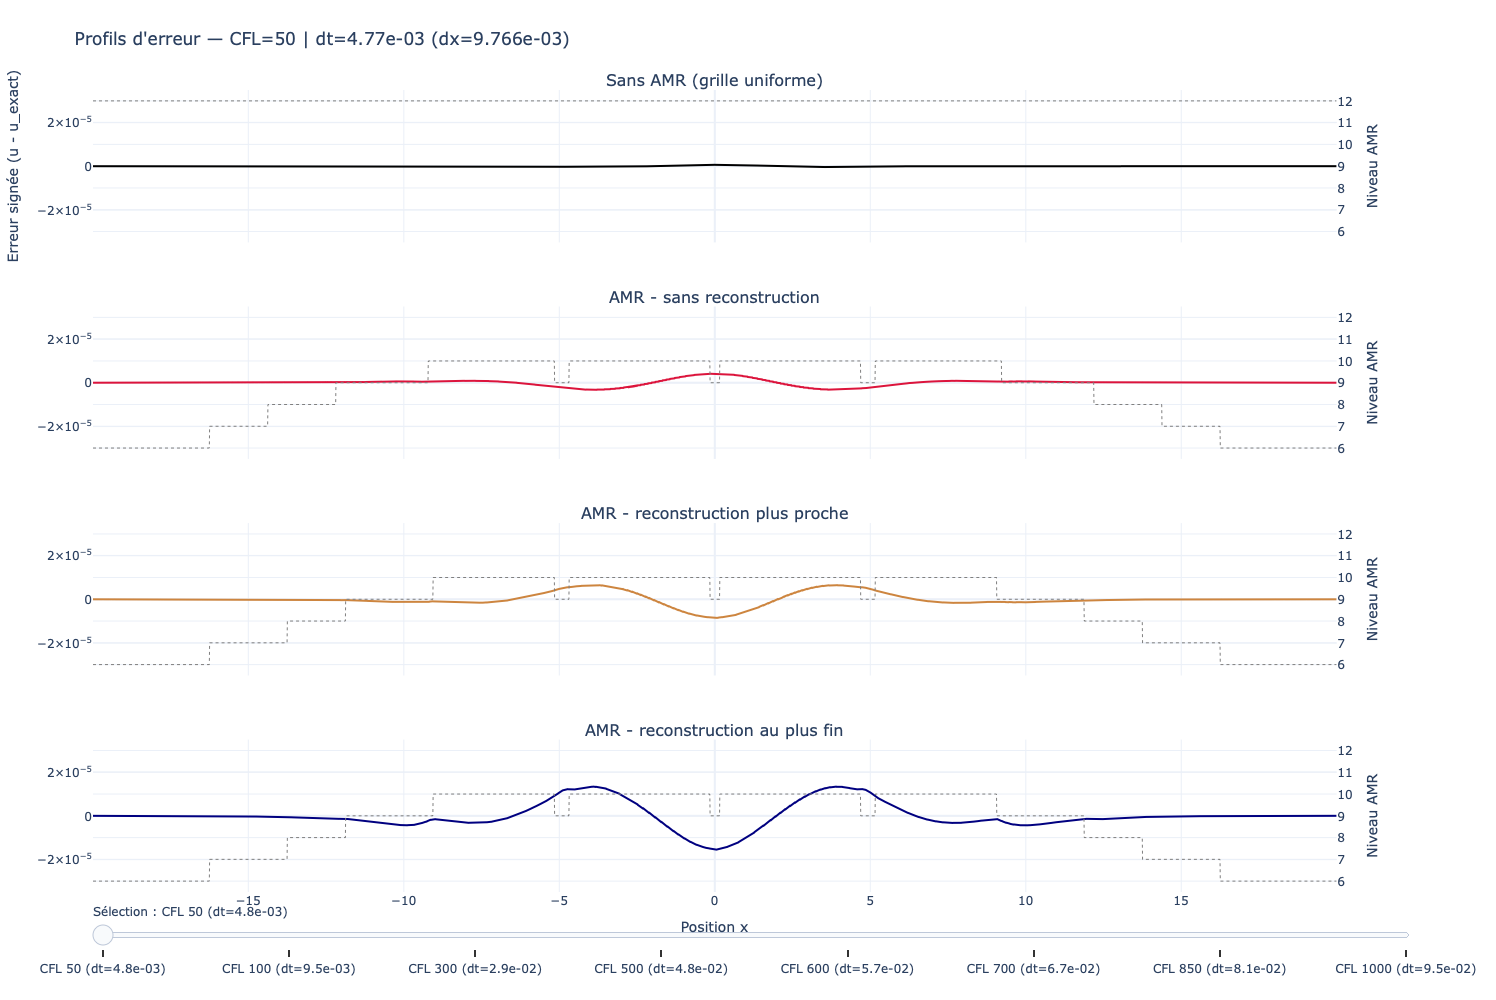
\includegraphics[width=\linewidth]{media/4_travail/3/03_error_profile_small_cfl.png}
    \subcaption{Constante CFL Petite}
\end{subfigure}

\caption{Profils d'erreur pour différentes valeurs de la constante CFL. C'est le pas d'espace est fixé, 
cela revient simplement à changer le pas de temps.}
\label{fig:error_profiles_landscape}
\end{minipage}%
}
\end{figure}
\clearpage
